\documentclass[12pt]{beamer}
\usetheme{Boadilla}
\usepackage{tikz}
\usepackage{pgfplots}
\renewcommand{\arraystretch}{1.25}
\usetikzlibrary{trees}
\title[ECON2843]{Lecture 3}
\subtitle{Part 1 Descriptive Statics, Summary Measures, and Data Visualization}
\date{}
\usepackage{amsmath,amssymb,mathtools,wasysym}
\begin{document}
	\begin{frame}
		\titlepage
	\end{frame}
\begin{frame}{Measures of Relative Standing}
	\begin{itemize}
		\item[$\blacktriangleright$] A {\bf measure of relative standing} measures the location of a particular value relative to the rest of the distribution of your data.
		\item[$\blacktriangleright$] Suppose you order your data from smallest to largest. A {\bf quantile} is the value below which a certain proportion (say $p$) of your data lie and above which one minus that proportion (i.e., $1-p$) of your data lie.
	\end{itemize}
\end{frame}
\begin{frame}{Examples of Quantiles}
	\begin{itemize}
		\item[$\blacktriangleright$] {\bf Quartiles} divide the data into quarters, and report the observation at the boundaries of the subsets.
		\begin{itemize}
		 \item For example, the first quartile ($Q_1$) is the value below which 25\% of your data lie, the second quartile ($Q_2$) is the value below which 50\% of your data lie, etc.
		 \end{itemize}
		\item[$\blacktriangleright$] {\bf Percentiles} divide the data into hundredths, and report the observation at the boundaries of the subsets.
		\begin{itemize}
			\item For example, the 91st percentile is the value below which 91\% of your data lie (and the value above which 9\% of your data lie).
		\end{itemize}
	\end{itemize}
\end{frame}
\begin{frame}{Calculating Percentiles}
	\begin{itemize}
		\item[$\blacktriangleright$] If we have $n$ observations, the location of the $p$th percentile is given by:
		$$L_p=(n+1)\frac{p}{100}$$
		\item[$\blacktriangleright$] Find the 31st percentile of the quiz marks from tutorial session A:
			\begin{center}
			\begin{tabular}{ccccccccc}
				\hline\hline
				A & 5 & 5 & 6 & 7 & 7 & 8 & 8 & 8\\
				\hline\hline
			\end{tabular}
		\end{center}
	\end{itemize}
\end{frame}
\begin{frame}{Calculating Percentiles}
	\begin{center}
		\begin{tabular}{ccccccccc}
			\hline\hline
			A & 5 & 5 & 6 & 7 & 7 & 8 & 8 & 8\\
			\hline\hline
		\end{tabular}
	\end{center}
	\begin{itemize}
		\item[$\blacktriangleright$] The location of the 31st percentile is:
		$$L_p=(8+1)\frac{31}{100}=2.79$$
		\item[$\blacktriangleright$] So the 31st percentile lies 0.79 of the distance between the 2nd and 3rd observations, which are 5 and 6, respectively.
		\item[$\blacktriangleright$] Therefore, the 31st percentile is equal to:
		$$5+(0.79)\times(6-5)=5.79$$
	\end{itemize}
\end{frame}
\begin{frame}{Interquartile Range}
	\begin{itemize}
		\item[$\blacktriangleright$] The interquartile range (IQR) of a data set is defined to be:
		$$\text{IQR}=Q_3-Q_1$$
			\begin{center}
			\begin{tabular}{ccccccccc}
				\hline\hline
				A & 5 & 6 & 5 & 7 & 8 & 7 & 8 & 8\\
				\hline
				B & 9 & 5 & 6 & 7 & 7 & 6 & 5 & \\
				\hline
			\end{tabular}
		\end{center}
		\vspace{0.5cm}
		
		\item[$\blacktriangleright$] Tutorial A: The IQR is $79.25-70.75 = 8.5$.
		\item[$\blacktriangleright$] Tutorial B: The IQR is $98-52 = 46$.
		\item[$\blacktriangleright$] IQR is more stable than the range.
	\end{itemize}
\end{frame}
\begin{frame}{Histograms}
	\begin{itemize}
		\item[$\blacktriangleright$] {\bf Histograms} plot the frequency of observations falling into defined intervals.
		\item[$\blacktriangleright$] Are one of the most useful ways to graphically present continuous data.
		\item[$\blacktriangleright$] Can give us information about the distribution of our data, including:
		\begin{itemize}
		\item The approximate location of the mean and median.
		\item The amount of spread/variability in our data.
		\item The shape of the distribution, e.g., skewness.
	    \end{itemize}
	\end{itemize}
\end{frame}
\begin{frame}{Histograms}
	
	Constructing a histogram:
	\begin{itemize}
		\item[$\blacktriangleright$] Determine the range of the data, i.e., the smallest and largest values of the variable.
		\item[$\blacktriangleright$] Divide the range into an appropriate number of intervals or "classes".
		\item[$\blacktriangleright$] Count the number of observations that fall into each interval.
		\item[$\blacktriangleright$] Plot the intervals on the $x$-axis and the frequency (count) for each interval on the $y$-axis.
	\end{itemize}
\end{frame}
\begin{frame}{Histograms}
	
	\begin{itemize}
		\item[$\blacktriangleright$] How many intervals should we use?
		\item[$\blacktriangleright$] Depends on the number of observations.
		\item[$\blacktriangleright$] Typically, more observations means we should use more intervals to have a nice-looking histogram.
		\item[$\blacktriangleright$] Plot the intervals on the $x$-axis and the frequency (count) for each interval on the $y$-axis.
	\end{itemize}
\end{frame}
\begin{frame}{Histograms}
	
	\begin{itemize}
		\item[$\blacktriangleright$] Back to favorite color example: Suppose while asking about favorite color, we also measured the height of each of student.
		\item[$\blacktriangleright$] Some descriptive statistics:
	\end{itemize}
		\begin{center}
		\begin{tabular}{cccccccc}
			\hline
			$n$ & $\bar{X}$ &$s$&Min &$Q_1$&Median&$Q_3$&Max\\
			\hline
			206 & 173.1 &8.96& 151.2& 167.3&172.4&178.5&203.6\\
			\hline
		\end{tabular}
	\end{center}
\end{frame}
\begin{frame}{Histograms}
\centering
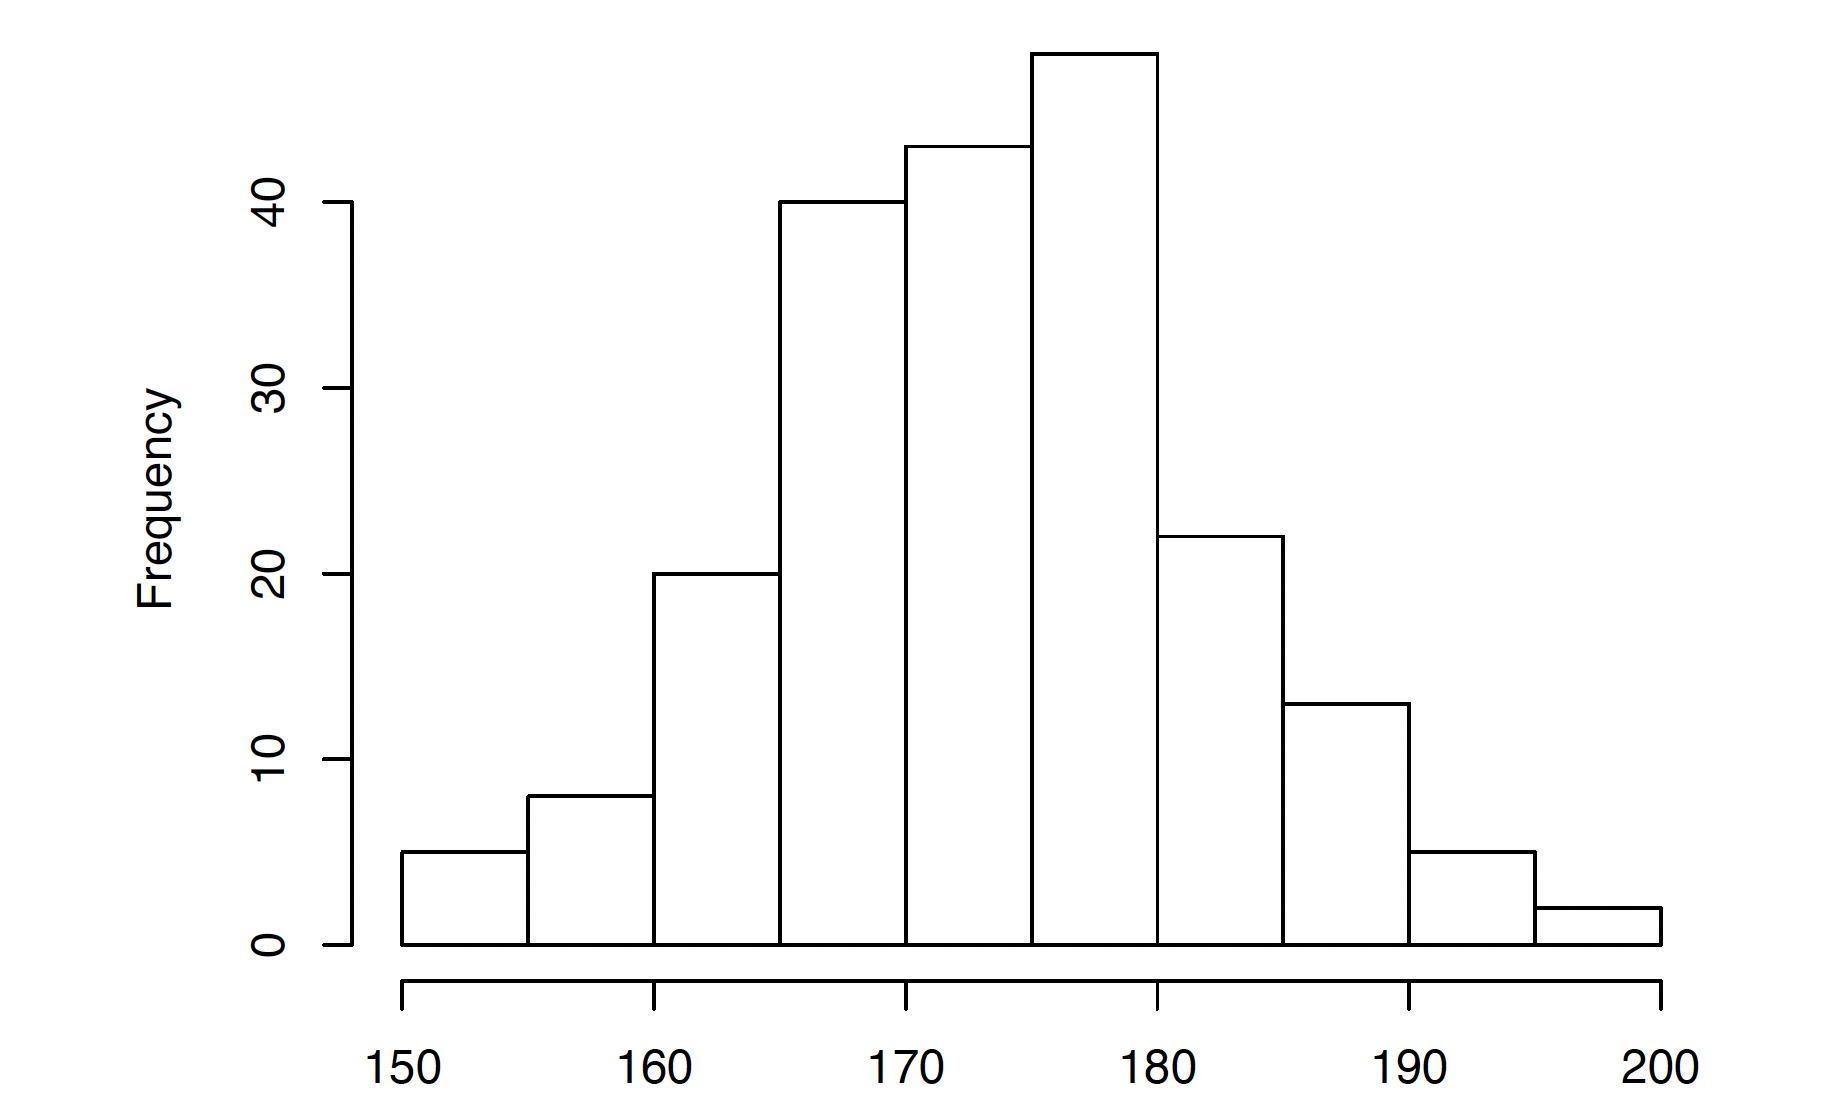
\includegraphics[width=12cm]{histo1.png}
\end{frame}
\begin{frame}{Histograms}
	
From a histogram, we can easily determine:
	\begin{itemize}
	\item[$\blacktriangleright$] The modal class, which is the class with the most observations.
	\item[$\blacktriangleright$] Whether the distribution of the data is uni-modal (one main peak in histogram) or multi-modal (multiple distinct peaks in histogram).
	\item[$\blacktriangleright$] Whether the distribution of the data is {\bf skewed} or {\bf symmetric}.
\end{itemize}
\end{frame}
\begin{frame}{Bimodal Distribution}
	\centering
	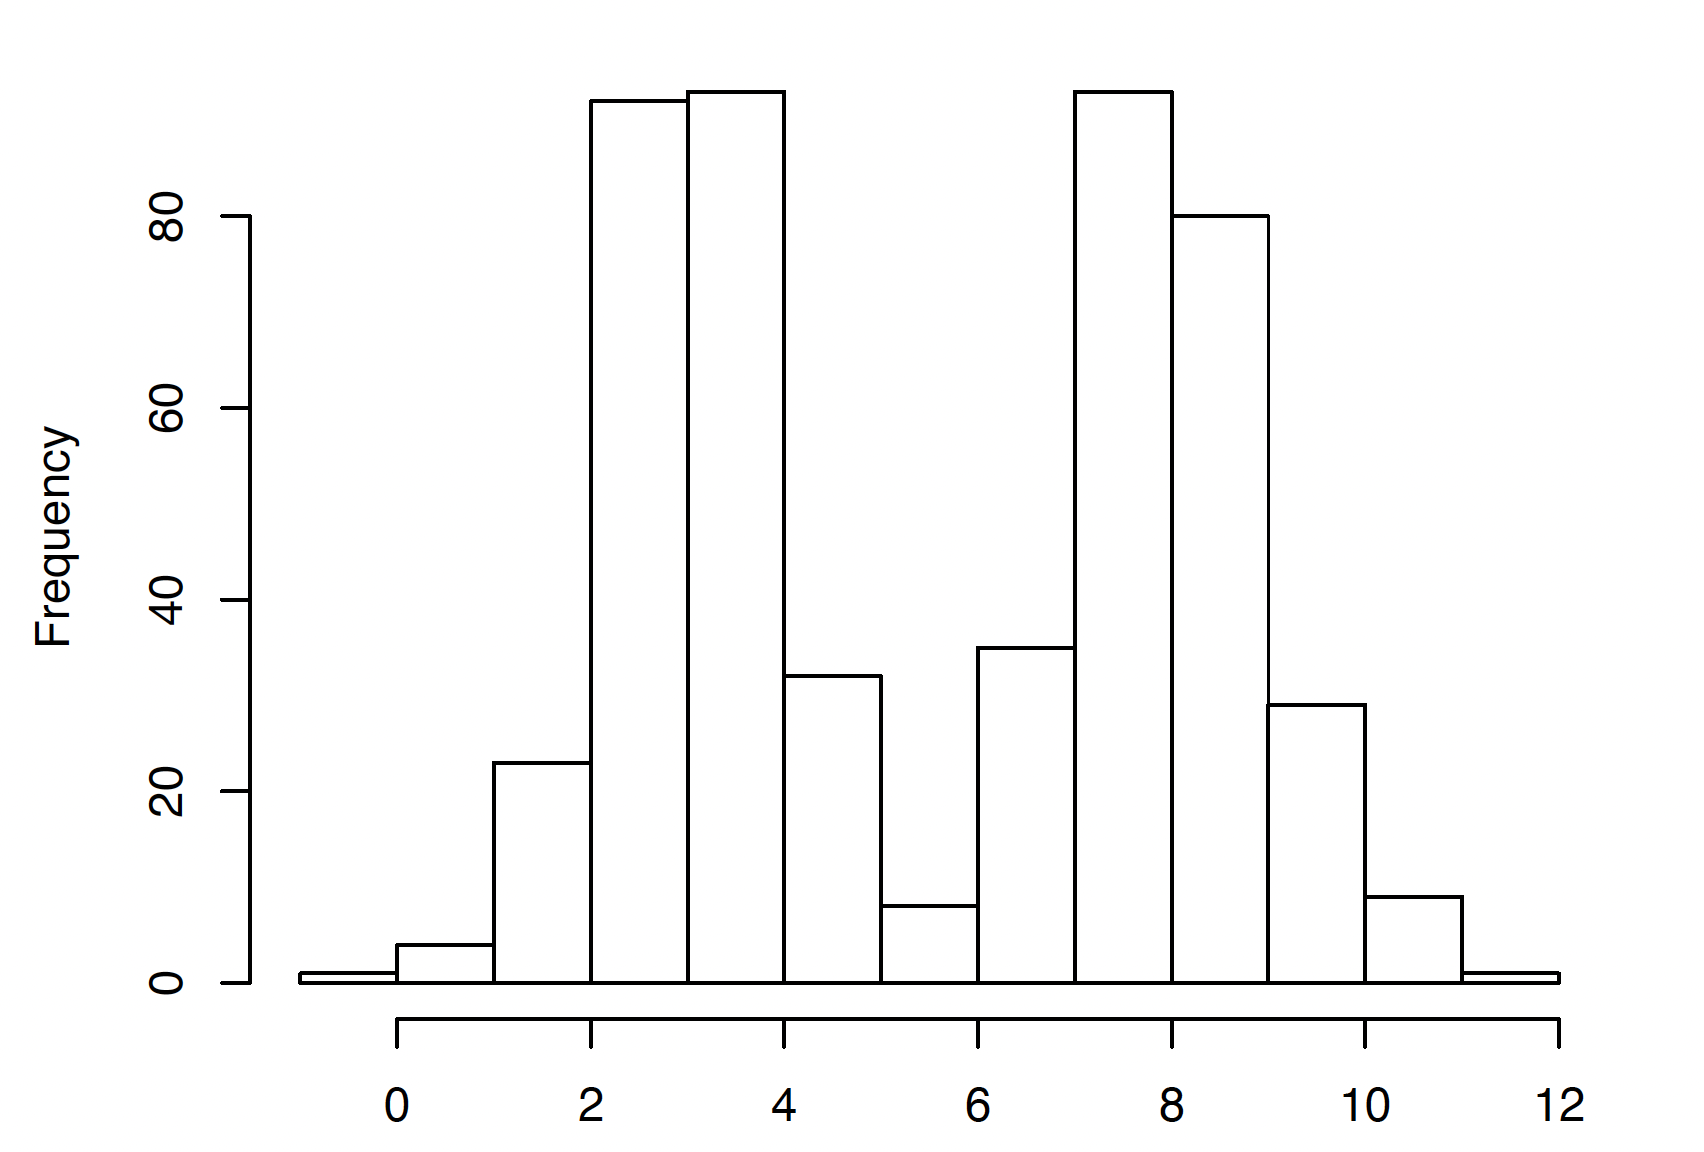
\includegraphics[width=12cm]{bimodal.png}
\end{frame}
\begin{frame}{Symmetric Distribution}
	\begin{itemize}
		\item[$\blacktriangleright$] {\bf Skewness} is a measure of asymmetry in a given distribution.
		\item[$\blacktriangleright$] If a distribution is symmetric, then the skewness is 0 and the mean is equal to the median.
	\end{itemize}
	\centering
	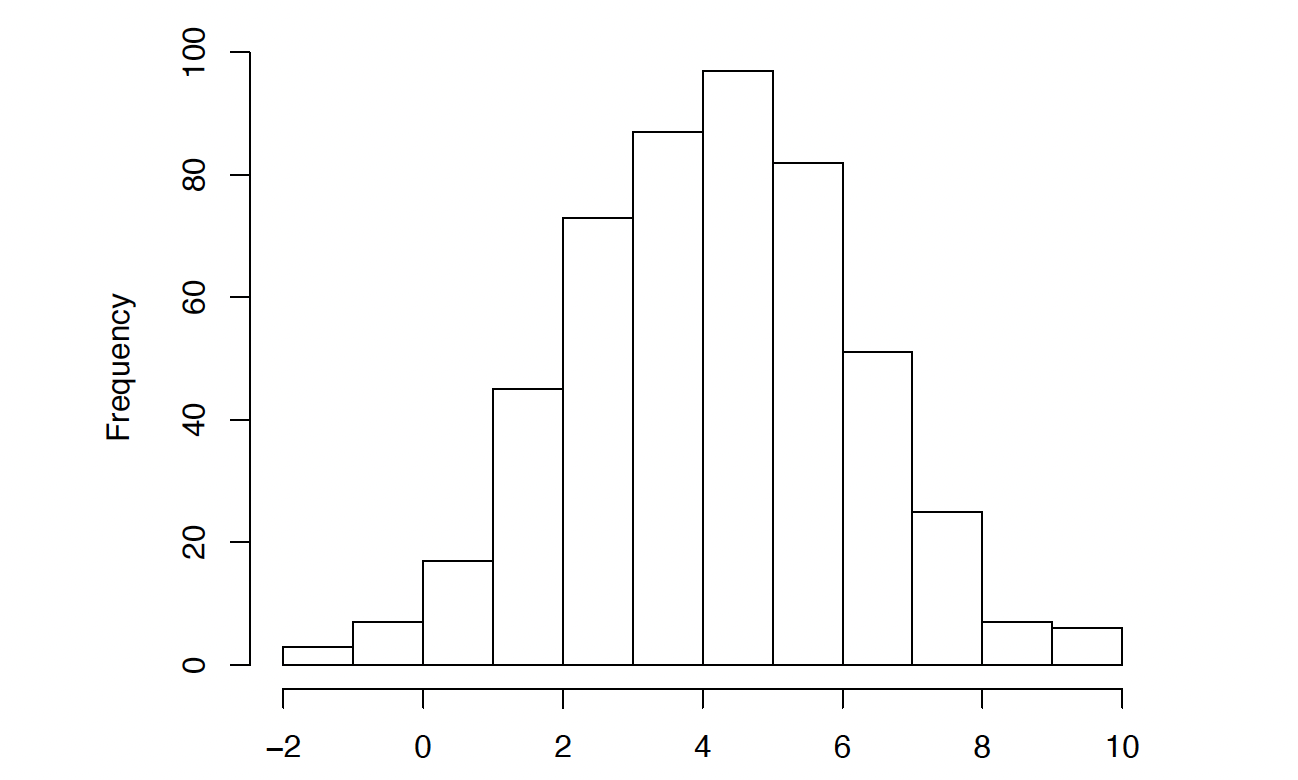
\includegraphics[width=10cm]{symme.png}
\end{frame}
\begin{frame}{Positively Skewed Distribution}
	\begin{itemize}
		\item[$\blacktriangleright$] If a distribution is positively skewed (or skewed to the right), then the mean is usually bigger than the median and the histogram will have a long tail to the right.
	\end{itemize}
	\centering
	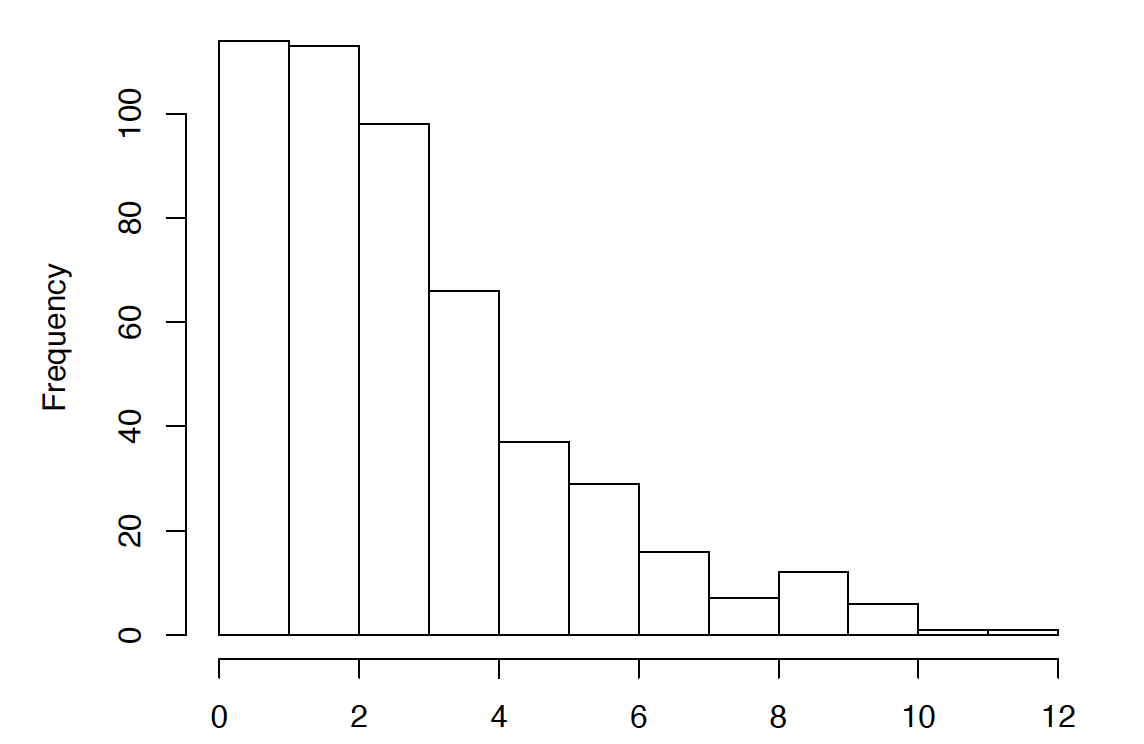
\includegraphics[width=10cm]{ps.png}
\end{frame}
\begin{frame}{Positively Skewed Distribution: Examples}
	\begin{itemize}
		\item[$\blacktriangleright$] Income Distribution: In many countries, a small number of people have very high incomes compared to the majority. This creates a long tail on the right side of the income distribution curve.
		\item[$\blacktriangleright$] Real Estate Prices: Housing prices can be positively skewed, with most homes priced in a lower range, but a few very expensive properties stretching the price distribution to the right.
		\item[$\blacktriangleright$] Time to Complete a Task: If most people complete a task relatively quickly but a few take significantly longer, the distribution of completion times might be positively skewed.
		
	\end{itemize}
\end{frame}
\begin{frame}{Negatively Skewed Distribution}
	\begin{itemize}
		\item[$\blacktriangleright$] If a distribution is negatively skewed (or skewed to the left), then the mean is usually smaller than the median and the histogram will have a long tail to the left.
	\end{itemize}
	\centering
	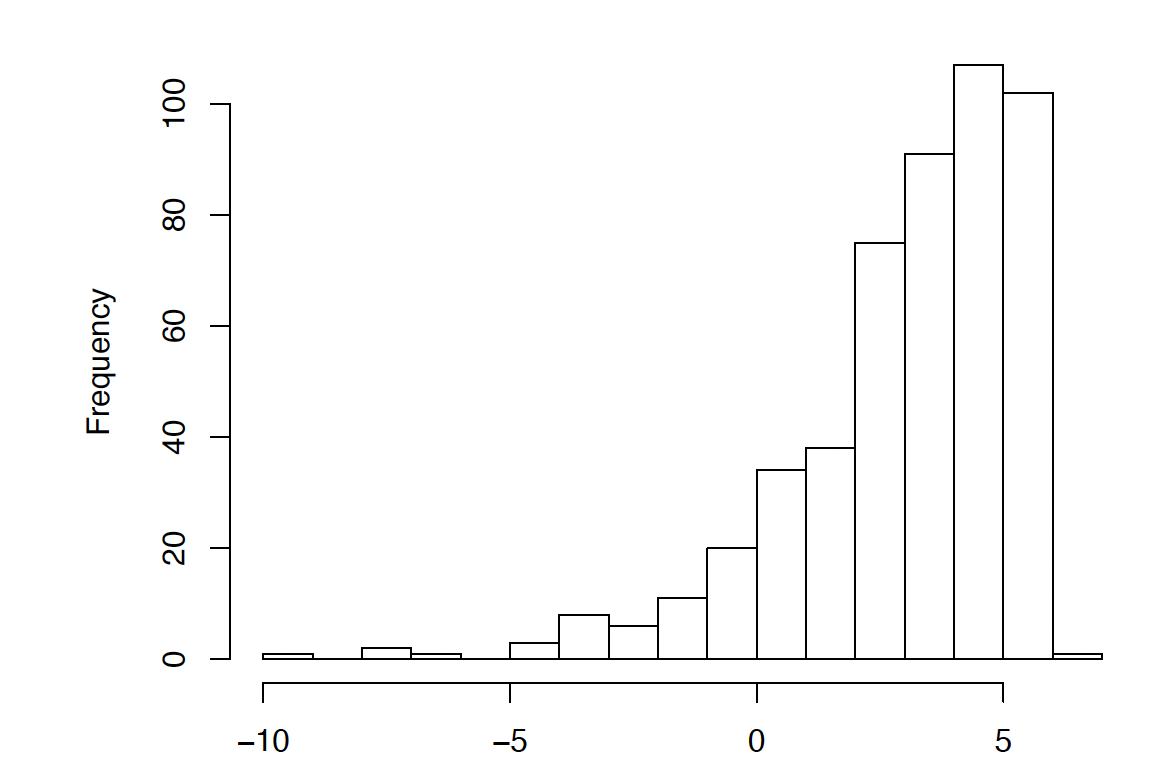
\includegraphics[width=10cm]{ns.png}
\end{frame}
\begin{frame}{Negatively Skewed Distribution: Examples}
	\begin{itemize}
		\item[$\blacktriangleright$] Survival Time of Cancer Patients: For a certain type of cancer, most patients may survive for many years after diagnosis (e.g., 5-10 years), but some patients may pass away shortly after diagnosis. This results in a negatively skewed distribution of survival time.
		\item[$\blacktriangleright$] Debt Repayment Time: Among debtors, most people may repay their debt close to or by the due date, but a small portion might repay their debt much earlier, leading to a negatively skewed distribution of repayment time.
		
	\end{itemize}
\end{frame}
\begin{frame}{Boxplots}
	\begin{itemize}
		\item[$\blacktriangleright$] Boxplots are another way to display continuous data.
		\item[$\blacktriangleright$] They can be useful, but do not provide as much information as a histogram.
		\item[$\blacktriangleright$] Based on five main statistics:
		\begin{itemize}
			\item The minimum and maximum observations.
			\item The first quartile $Q_1$, the median $Q_2$ and the third quartile $Q_3$.
		\end{itemize}
	\item[$\blacktriangleright$] And they look like...
	\end{itemize}
\end{frame}
\begin{frame}{Boxplots}
\centering
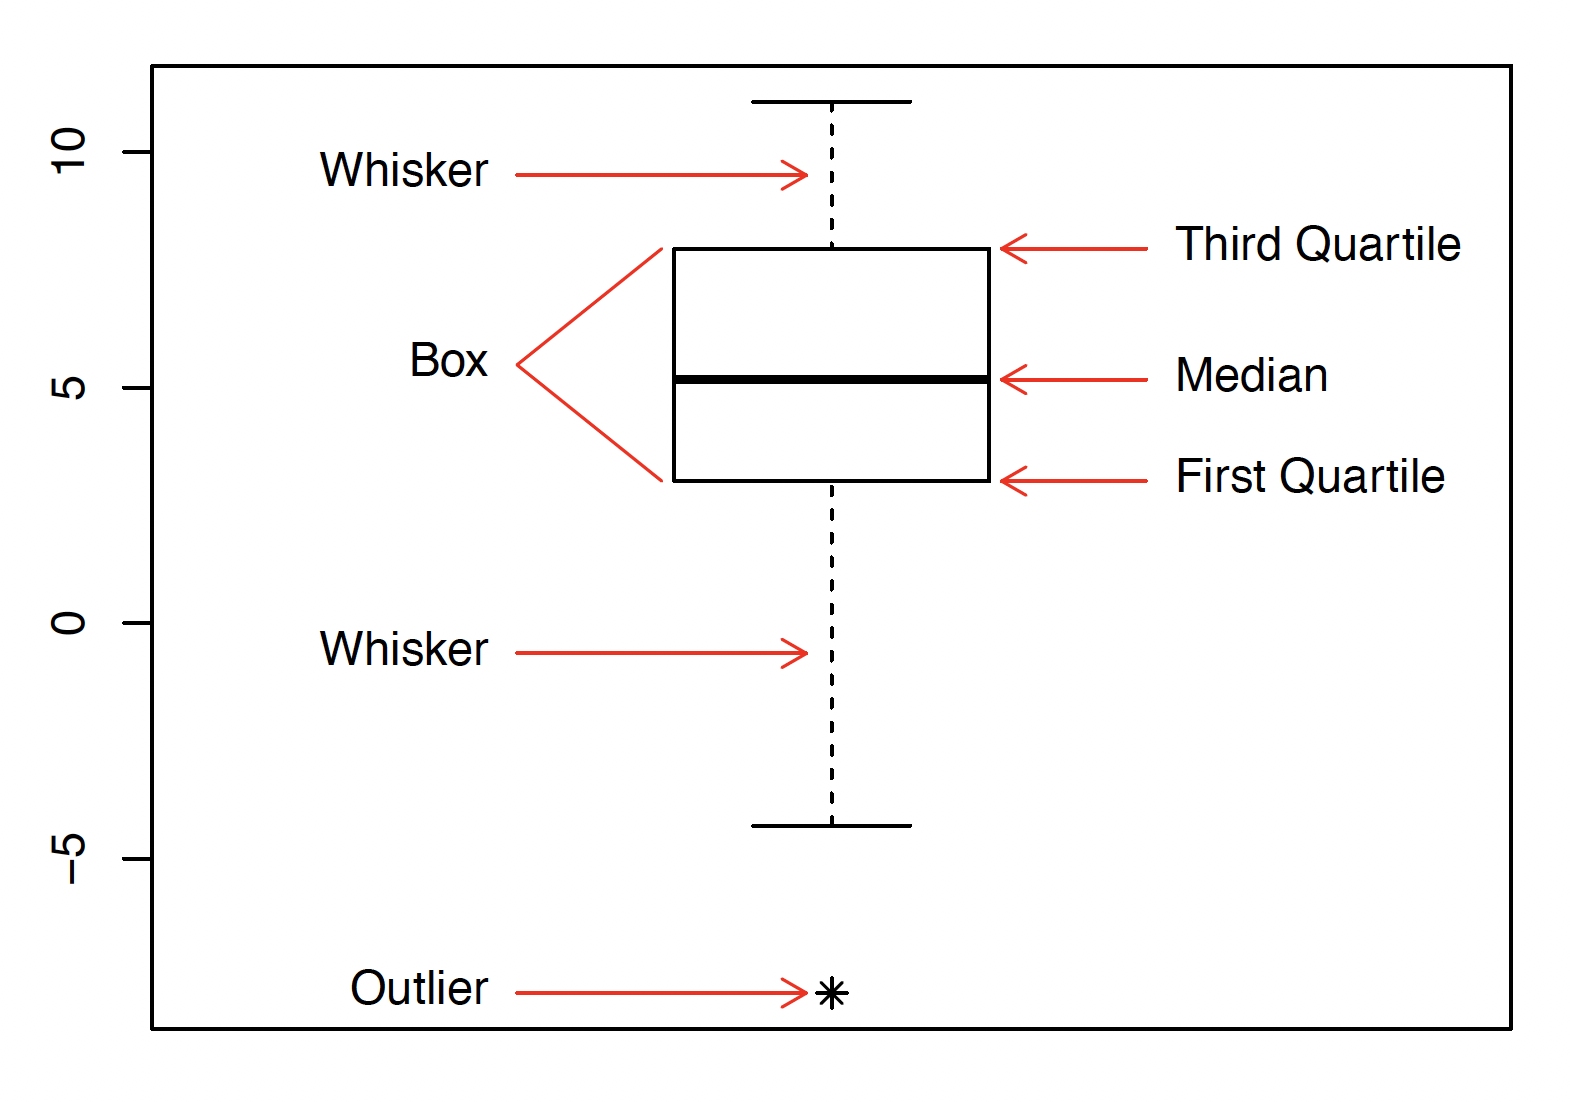
\includegraphics[width=10cm]{box.png}
\end{frame}
\begin{frame}{Boxplots}
	
	Constructing a boxplot:
\begin{itemize}
	\item[$\blacktriangleright$] Draw three lines at $Q_1$, the median and $Q_3$. These three lines will form the box.
	\item[$\blacktriangleright$] Calculate the interquartile range (IQR).
	\item[$\blacktriangleright$] Draw a line that extends from the first quartile to either the smallest observation or 1.5 times the IQR, whichever distance is shorter, and from the third quartile to either the largest observation or 1.5 times the IQR, whichever distance is shorter.
	\item[$\blacktriangleright$] These two lines drawn then form the whiskers.
	\item[$\blacktriangleright$] Any observations which lie further outside these whiskers are marked with stars and are called outliers.
\end{itemize}
\end{frame}
\begin{frame}{Boxplots}
	\centering
	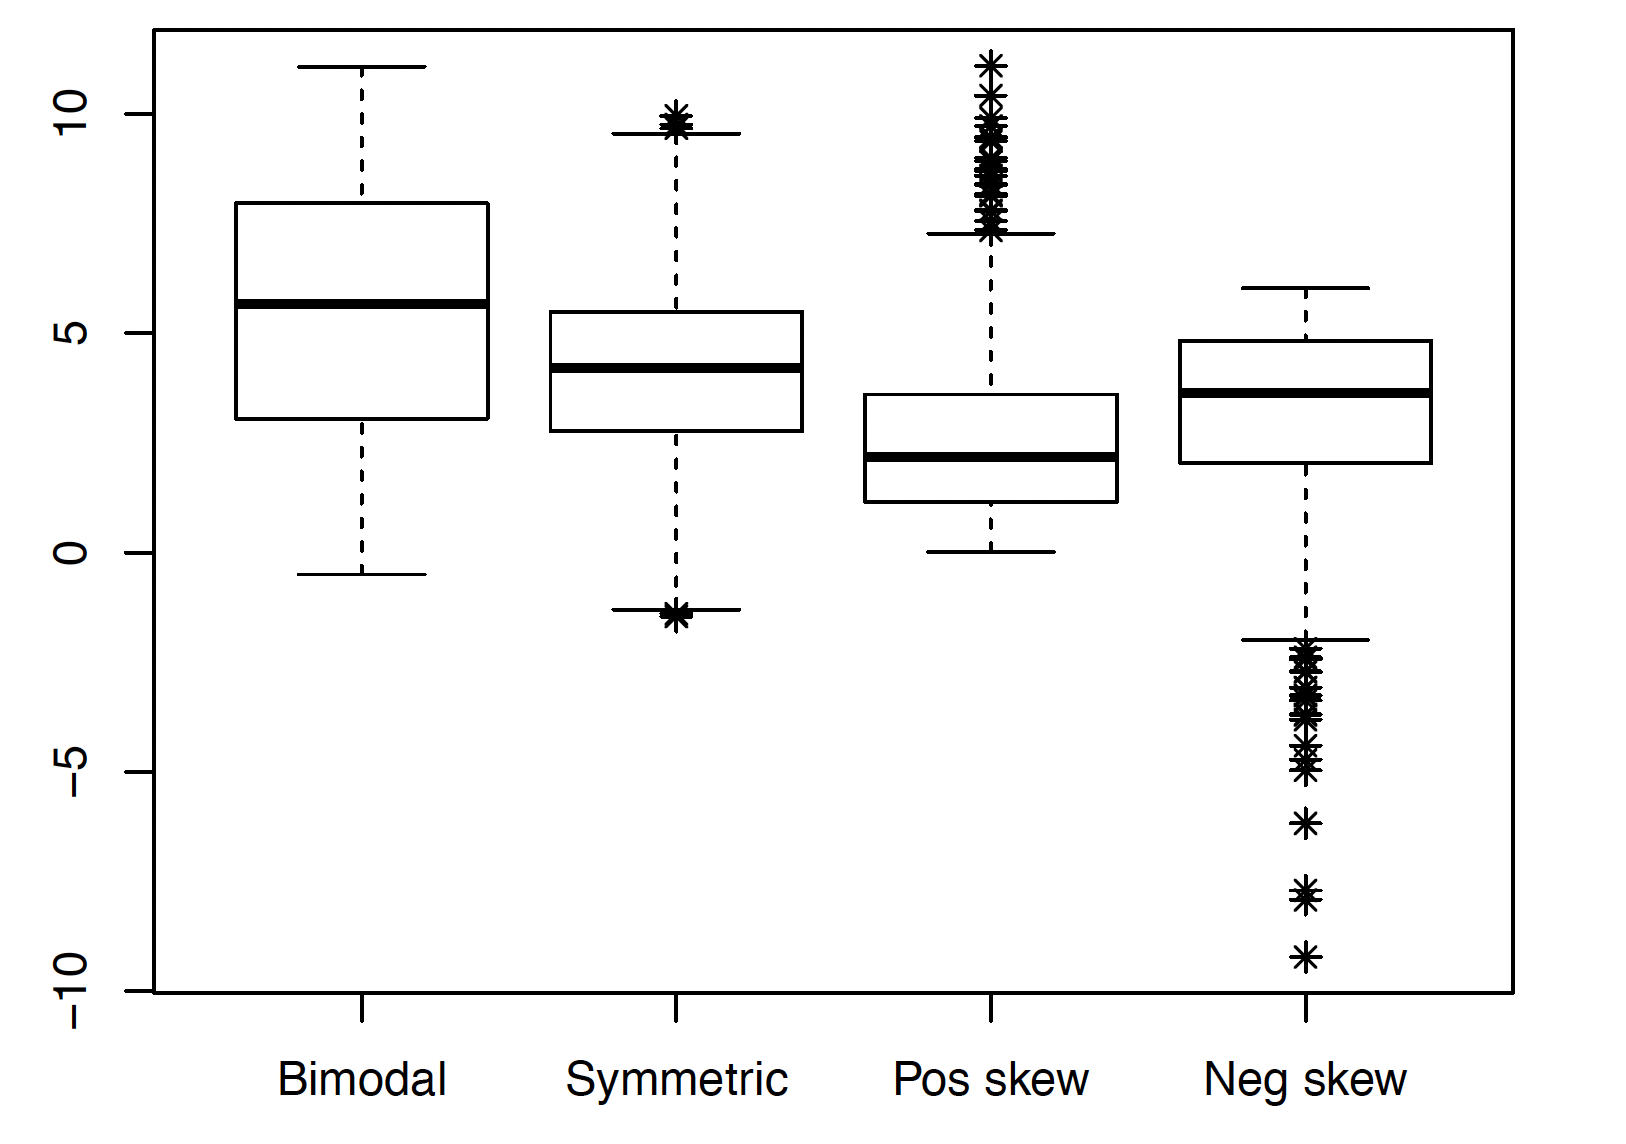
\includegraphics[width=10cm]{box2.png}
\end{frame}
\end{document}